\documentclass[11pt,a4paper]{article}

\usepackage[margin=1in]{geometry}
\usepackage{graphicx}
\usepackage{booktabs}
\usepackage{amsmath}
\usepackage{amssymb}
\usepackage{siunitx}
\usepackage{hyperref}
\usepackage{setspace}
\usepackage{enumitem}
\usepackage{xcolor}
\usepackage{listings}
\usepackage{float}
\usepackage{tikz}
\usetikzlibrary{shapes.geometric, arrows.meta, positioning, fit, calc}

\hypersetup{
    colorlinks=true,
    linkcolor=black,
    urlcolor=blue,
    citecolor=black
}

\sisetup{
    group-separator={,}
}

\lstset{
    basicstyle=\ttfamily\small,
    keywordstyle=\color{blue}\bfseries,
    commentstyle=\color{gray}\itshape,
    stringstyle=\color{red!70!black},
    backgroundcolor=\color{gray!5},
    frame=single,
    framerule=0.4pt,
    rulecolor=\color{gray!50},
    breaklines=true,
    showstringspaces=false,
    tabsize=4,
    captionpos=b,
    numbers=left,
    numberstyle=\tiny\color{gray},
    numbersep=8pt,
    xleftmargin=2em,
    language=Python,
}

\title{\textbf{Intelligent Real Estate Advisory System}\\[4pt]
\large ML Prediction, RAG, and LangGraph Agent Workflow\\[2pt]
\normalsize Ames Housing Dataset}
\author{
Kavya Katal \and
Aabir Sarkar \and
Kushagra Maheswari \and
Pratyush Chouksey
}
\date{\today}

\begin{document}
\maketitle

\onehalfspacing

\begin{abstract}
This project presents an intelligent real estate advisory system that integrates Machine Learning (ML), Retrieval-Augmented Generation (RAG), and an agentic workflow orchestrated by LangGraph.
The system predicts residential property prices from the Ames Housing dataset using a scikit-learn Linear Regression pipeline with a log-transformed target, achieving an R\textsuperscript{2} of 0.93 and MAE of \$14,899 on the validation set.
Beyond numerical prediction, a three-node LangGraph agent enriches the output by retrieving market context from a ChromaDB vector store via sentence-transformer embeddings, performing comparable-property analysis against the historical dataset, and generating a structured advisory report through an LLM served by OpenRouter.
A deterministic rule-based fallback guarantees advisory availability when the LLM is unreachable.
The entire pipeline is deployed as an interactive Streamlit web application, providing users with price estimates, market insights, and investment recommendations in a single interface.
\end{abstract}

\tableofcontents
\newpage

% =========================================================
%  PART I — MACHINE LEARNING PIPELINE
% =========================================================

\part{Machine Learning Pipeline}

% -------------------------------------------------
% 1. Problem Statement
% -------------------------------------------------
\section{Problem Statement}

Buying or selling a house involves high-stakes financial decisions.
However, manually estimating a fair market value is difficult because property prices depend on a large number of factors such as neighbourhood, living area, construction quality, age, and amenities.
Traditional appraisal methods are labour-intensive, subjective, and hard to scale.

\textbf{Goal:}
Given structured information about a residential property, we aim to automatically predict its sale price (in USD) using supervised machine learning.
The model should:

\begin{itemize}[leftmargin=*]
    \item Produce \textbf{reasonably accurate and stable} price estimates on unseen properties.
    \item \textbf{Generalise} beyond the training data without overfitting.
    \item Be \textbf{fast and lightweight} enough to support an interactive web interface.
    \item Be \textbf{interpretable and maintainable}, with a clear preprocessing pipeline and reproducible training process.
\end{itemize}

\noindent
\textbf{Scope:}
The project focuses on predicting prices for properties in the Ames, Iowa housing market using historical sales data.
While the deployed Streamlit app exposes only a subset of features to the user (e.g., overall quality, living area, basement area, year built), the underlying training pipeline handles the full feature set of the dataset.

% -------------------------------------------------
% 2. Data Description
% -------------------------------------------------
\section{Data Description}

\subsection{Dataset Origin}

We use the \textbf{Ames Housing} dataset, popularised via the Kaggle competition ``House Prices: Advanced Regression Techniques''.
The dataset contains detailed information about residential property sales in Ames, Iowa.

\begin{itemize}[leftmargin=*]
    \item \textbf{Source:} Kaggle / Ames Housing public dataset.
    \item \textbf{File used:} A large tabular CSV (referred to as \texttt{BigHousing.csv} in this repository).
    \item \textbf{Target variable:} \texttt{SalePrice} (USD).
\end{itemize}

\subsection{Feature Overview}

The raw dataset contains around 80 input features describing each property.
These features fall into the following broad categories:

\begin{itemize}[leftmargin=*]
    \item \textbf{Physical characteristics}
    \begin{itemize}
        \item \texttt{GrLivArea}: Above-ground living area (square feet).
        \item \texttt{TotalBsmtSF}: Basement area (square feet).
        \item \texttt{LotArea}: Lot size (square feet).
        \item \texttt{BsmtFullBath}, \texttt{FullBath}: Number of bathrooms.
        \item \texttt{GarageCars}: Garage capacity (number of cars).
        \item \texttt{Fireplaces}: Number of fireplaces.
    \end{itemize}
    \item \textbf{Quality and condition}
    \begin{itemize}
        \item \texttt{OverallQual}: Overall material and finish quality (1--10).
        \item \texttt{OverallCond}: Overall condition rating.
        \item Exterior/interior material quality ratings (e.g.\ \texttt{ExterQual}, \texttt{KitchenQual}).
    \end{itemize}
    \item \textbf{Age and year-related variables}
    \begin{itemize}
        \item \texttt{YearBuilt}: Original construction date.
        \item \texttt{YearRemodAdd}: Remodel date.
        \item \texttt{YrSold}: Year sold.
    \end{itemize}
    \item \textbf{Location and configuration}
    \begin{itemize}
        \item \texttt{Neighborhood}: Physical location within Ames.
        \item \texttt{MSZoning}: General zoning classification.
        \item \texttt{HouseStyle}, \texttt{BldgType}: Building and house style.
    \end{itemize}
\end{itemize}

In our training pipeline, we automatically infer column types:

\begin{itemize}[leftmargin=*]
    \item \textbf{36 numeric} columns (floats/integers).
    \item \textbf{43 categorical} columns (strings or categories).
\end{itemize}

The \texttt{Id} column is an identifier and is dropped before training.

\subsection{Target Variable}

The target is the final sale price of each property:

\begin{itemize}[leftmargin=*]
    \item \textbf{Name:} \texttt{SalePrice}
    \item \textbf{Unit:} USD
    \item \textbf{Type:} Continuous numeric
\end{itemize}

As explored in Section~\ref{sec:eda-target}, \texttt{SalePrice} is right-skewed, motivating a log-transformation during model training.

% -------------------------------------------------
% 3. EDA Process
% -------------------------------------------------
\section{EDA Process}

Our exploratory data analysis (EDA) was performed primarily in a Jupyter notebook and guided the preprocessing and modelling choices.

\subsection{Dataset Audit and Structure}

We first examined the basic structure of the dataset:

\begin{itemize}[leftmargin=*]
    \item Checked the shape: approximately 1460 rows and 80+ features.
    \item Inspected column data types to separate numeric and categorical variables.
    \item Verified that the \texttt{SalePrice} column (target) exists and has no missing values.
    \item Confirmed the presence of both continuous measurements (e.g., square footage) and many categorical descriptors (e.g., neighbourhood, exterior material).
\end{itemize}

\subsection{Missing Values and Data Quality}

We computed the count of missing values per column and sorted them in descending order.
Several features exhibited substantial missingness, especially optional attributes such as \texttt{Alley}, \texttt{PoolQC}, and some basement/garage features.

\subsection{Target Distribution and Transformation}
\label{sec:eda-target}

The raw distribution of \texttt{SalePrice} is strongly right-skewed, with a long tail of expensive properties.
This violates the normality assumption underlying many regression models and can cause models to underperform on typical houses or be overly influenced by outliers.

Using the notebook, we visualised the histogram of \texttt{SalePrice} and then the histogram of \(\log(1 + \texttt{SalePrice})\).
The log-transformed target is much closer to a symmetric, approximately normal distribution, which stabilises training and improves model fit.

\subsection{Correlation Analysis}

We computed the Pearson correlation between numeric features and the target (in USD) and plotted the 12 most correlated numeric features.

Key observations:

\begin{itemize}[leftmargin=*]
    \item \textbf{Overall quality (\texttt{OverallQual})} has one of the strongest positive correlations with \texttt{SalePrice}.
    \item \textbf{Living area (\texttt{GrLivArea})} and \textbf{basement area} (\texttt{TotalBsmtSF}) are also highly correlated.
    \item \textbf{Garage capacity} (\texttt{GarageCars}) and \textbf{year built} (\texttt{YearBuilt}) show meaningful positive correlations.
\end{itemize}

These insights motivated both the choice of input features highlighted in the Streamlit UI and the expectation that a mostly linear model might perform well after appropriate transformations.

\subsection{Train--Validation Split}

To obtain unbiased estimates of model performance, we split the dataset into training and validation sets:

\begin{itemize}[leftmargin=*]
    \item \textbf{Train:} 80\% of the data.
    \item \textbf{Validation:} 20\% of the data.
    \item \textbf{Random seed:} 42 (for reproducibility).
\end{itemize}

This split results in 1168 training examples and 292 validation examples.
The same split is used for all model comparisons to ensure fairness.

% -------------------------------------------------
% 4. Methodology
% -------------------------------------------------
\section{Methodology}

\subsection{Overall Pipeline Design}

Instead of manually cleaning and transforming features in an ad hoc manner, we use a \textbf{scikit-learn pipeline} based on \texttt{ColumnTransformer} and \texttt{Pipeline} objects.
This design has several advantages:

\begin{itemize}[leftmargin=*]
    \item Training and inference (in the Streamlit app) run the \textbf{exact same} preprocessing steps.
    \item Complex transformations are encapsulated and reproducible.
    \item The final model artifact can be serialised with joblib and loaded directly in production.
\end{itemize}

The high-level flow is:

\begin{enumerate}[leftmargin=*]
    \item Load and clean raw data.
    \item Separate features \(\mathbf{X}\) and target \(y = \texttt{SalePrice}\).
    \item Drop the \texttt{Id} column.
    \item Split into training and validation sets.
    \item Apply \(\log(1 + y)\) transformation to the target for training.
    \item Fit preprocessing + model pipelines on training data.
    \item Evaluate on the validation set, converting predictions back to USD using \(\exp(y_{\log}) - 1\).
    \item Save the final pipeline, target transform flag, and training column names as a joblib artifact.
\end{enumerate}

\subsection{Preprocessing for Numeric Features}

Numeric features are processed through the following steps:

\begin{itemize}[leftmargin=*]
    \item \textbf{Missing value imputation:} Replace missing values with the median of each column using \texttt{SimpleImputer(strategy="median")}.
    \item \textbf{Scaling (for Linear Regression):} Standardise features to zero mean and unit variance using \texttt{StandardScaler}.
\end{itemize}

For the Random Forest model, scaling is not required, so we only perform median imputation.

\subsection{Preprocessing for Categorical Features}

Categorical features undergo:

\begin{itemize}[leftmargin=*]
    \item \textbf{Most-frequent imputation:} Fill missing values with the most frequent category per column.
    \item \textbf{One-hot encoding:} Convert categorical values into binary indicator columns using \texttt{OneHotEncoder(handle\_unknown="ignore")}.
\end{itemize}

Using \texttt{handle\_unknown="ignore"} ensures that the model can safely process categories that did not appear during training (important in deployment).

\subsection{Target Transformation}

As established in Section~\ref{sec:eda-target}, the target \texttt{SalePrice} is right-skewed.
We therefore train models on:

\[
y_{\log} = \log(1 + \texttt{SalePrice})
\]

At prediction time, we invert this transformation to obtain prices in USD:

\[
\widehat{\texttt{SalePrice}} = \exp(y_{\log}^{\text{pred}}) - 1
\]

This transformation reduces the influence of extreme outliers, brings the target distribution closer to normal, and often improves both MAE and RMSE for regression tasks with heavy-tailed targets.
The transformation flag (\texttt{"log1p"}) is stored with the saved artifact so the Streamlit app can consistently apply the inverse transform via \texttt{numpy.expm1}.

\subsection{Baseline Model: Linear Regression}

We first build a baseline using ordinary least squares Linear Regression:

\begin{itemize}[leftmargin=*]
    \item \textbf{Model:} scikit-learn's \texttt{LinearRegression}.
    \item \textbf{Pipeline:} Numeric: median imputation + standard scaling. Categorical: most-frequent imputation + one-hot encoding. Regressor: Linear Regression trained on \(y_{\log}\).
\end{itemize}

\subsection{Comparison Model: Random Forest Regressor}

To capture potential non-linear relationships and interactions, we also train a Random Forest Regressor:

\begin{itemize}[leftmargin=*]
    \item \textbf{Model:} \texttt{RandomForestRegressor} with \texttt{n\_estimators = 600}, \texttt{random\_state = 42}, \texttt{n\_jobs = -1}, and default depth.
    \item \textbf{Pipeline:} Numeric: median imputation (no scaling). Categorical: most-frequent imputation + one-hot encoding. Regressor: Random Forest trained on \(y_{\log}\).
\end{itemize}

\subsection{Model Serialization and Deployment Artifacts}

After training, we save the artifacts using joblib:

\begin{itemize}[leftmargin=*]
    \item \textbf{Pipeline:} The final trained Linear Regression pipeline (preprocessing + model).
    \item \textbf{Target transform flag:} \texttt{"log1p"} to indicate the target was transformed.
    \item \textbf{Training columns:} The list of original feature columns expected by the pipeline.
\end{itemize}

These are stored in a single joblib file (\texttt{model/house\_price\_lr\_pipeline.joblib}) which is loaded by the Streamlit app.

% -------------------------------------------------
% 5. ML Evaluation
% -------------------------------------------------
\section{ML Model Evaluation}
\label{sec:ml-eval}

\subsection{Metrics}

We evaluate regression performance on the validation set using:

\begin{itemize}[leftmargin=*]
    \item \textbf{MAE (Mean Absolute Error):}
    \[
    \text{MAE} = \frac{1}{n} \sum_{i=1}^n \left| y_i - \hat{y}_i \right|
    \]
    \item \textbf{RMSE (Root Mean Squared Error):}
    \[
    \text{RMSE} = \sqrt{\frac{1}{n} \sum_{i=1}^n \left( y_i - \hat{y}_i \right)^2}
    \]
    \item \textbf{R\textsuperscript{2} (Coefficient of Determination):}
    \[
    R^2 = 1 - \frac{\sum_i (y_i - \hat{y}_i)^2}{\sum_i (y_i - \bar{y})^2}
    \]
\end{itemize}

All metrics are reported in the original price space (USD), after inverting the log-transform.

\subsection{Quantitative Results}

Table~\ref{tab:metrics} summarises the performance of both models on the validation set.

\begin{table}[H]
    \centering
    \caption{Validation performance of Linear Regression and Random Forest models.}
    \label{tab:metrics}
    \begin{tabular}{l
                    S[table-format=5.0]
                    S[table-format=5.0]
                    S[table-format=1.4]}
        \toprule
        \textbf{Model} & \textbf{MAE (USD)} & \textbf{RMSE (USD)} & \textbf{R\textsuperscript{2}} \\
        \midrule
        Linear Regression (log target) & 14899 & 22740 & 0.9326 \\
        Random Forest (log target)     & 17495 & 30153 & 0.8815 \\
        \bottomrule
    \end{tabular}
\end{table}

\subsection{Interpretation}

Despite being simpler, the Linear Regression model achieves a lower MAE and RMSE compared to the Random Forest, and explains a higher proportion of variance in prices (R\textsuperscript{2}~\(\approx 0.93\) vs.~0.88).
These results suggest that, after appropriate preprocessing and log-transforming the target, the relationship between the selected features and \texttt{SalePrice} is largely linear.
The more complex Random Forest model underperforms, likely because it overfits noise and does not benefit enough from modelling non-linearities at this dataset scale.

\subsection{Model Selection}

Based on the validation metrics and practical concerns (speed, interpretability, and ease of deployment), we select the \textbf{Linear Regression (log target)} pipeline as the final model for deployment.

\newpage
% =========================================================
%  PART II — RETRIEVAL-AUGMENTED GENERATION (RAG)
% =========================================================

\part{Retrieval-Augmented Generation (RAG)}

% -------------------------------------------------
% 6. RAG Motivation
% -------------------------------------------------
\section{Motivation for RAG}
\label{sec:rag-motivation}

While the ML model provides a numerical price prediction, real estate decisions require additional contextual reasoning: market trends, investment heuristics, risk factors, and domain knowledge.
Rather than embedding all this knowledge directly into the LLM prompt (which would be static, token-expensive, and difficult to maintain), we adopt a \textbf{Retrieval-Augmented Generation (RAG)} architecture.

RAG separates knowledge storage from reasoning:

\begin{enumerate}[leftmargin=*]
    \item A \textbf{knowledge base} of domain-specific documents is embedded into a vector store at ingestion time.
    \item At query time, the user's property context is encoded into the same embedding space, and the most semantically relevant documents are retrieved.
    \item The retrieved context is injected into the LLM prompt, grounding the model's advisory in factual, retrievable evidence.
\end{enumerate}

This architecture provides several advantages over a pure LLM approach:

\begin{itemize}[leftmargin=*]
    \item \textbf{Grounded responses:} The LLM reasons over retrieved evidence rather than relying solely on parametric memory, reducing hallucination.
    \item \textbf{Updatable knowledge:} New insights can be added to the vector store without retraining or modifying the LLM.
    \item \textbf{Transparency:} Retrieved documents serve as citable evidence, making the advisory auditable.
    \item \textbf{Cost efficiency:} Only the most relevant context is sent to the LLM, keeping token usage low.
\end{itemize}

% -------------------------------------------------
% 7. RAG Architecture
% -------------------------------------------------
\section{RAG Architecture}

\subsection{System Diagram}

Figure~\ref{fig:rag-arch} illustrates the RAG pipeline from knowledge ingestion through retrieval to prompt augmentation.

\begin{figure}[H]
\centering
\resizebox{\linewidth}{!}{%
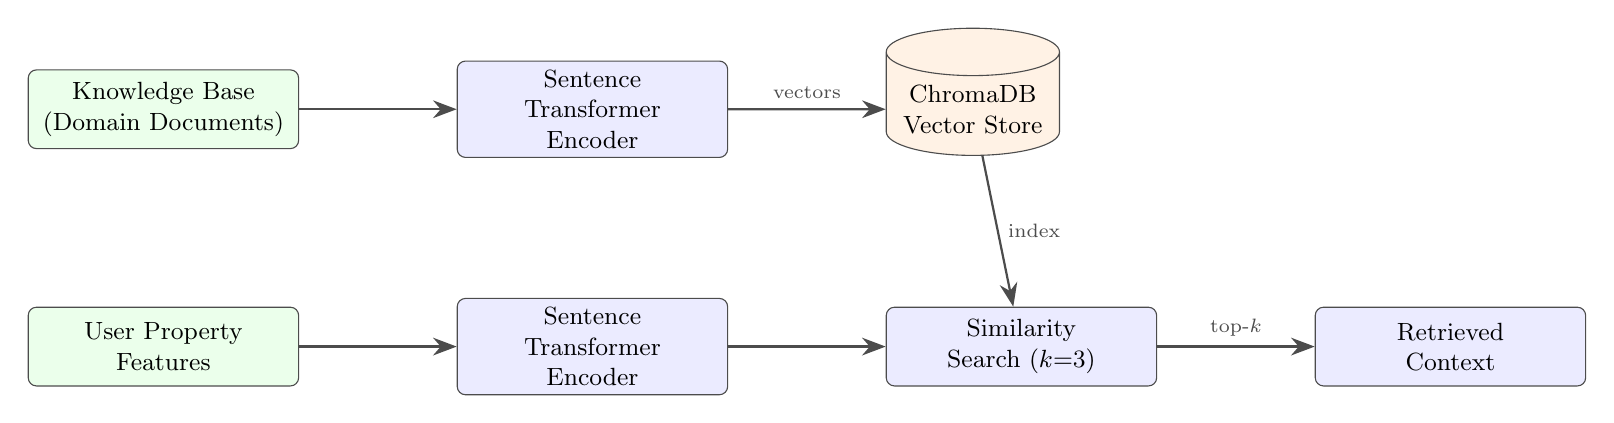
\begin{tikzpicture}[
    node distance=1.2cm and 2.0cm,
    block/.style={rectangle, draw=black!70, fill=blue!8, text width=3.2cm, minimum height=1cm, align=center, rounded corners=3pt, font=\small},
    data/.style={rectangle, draw=black!70, fill=green!8, text width=3.2cm, minimum height=1cm, align=center, rounded corners=3pt, font=\small},
    store/.style={cylinder, draw=black!70, fill=orange!10, shape border rotate=90, aspect=0.3, minimum height=1.2cm, minimum width=2.2cm, align=center, font=\small},
    arrow/.style={-{Stealth[length=3mm]}, thick, color=black!70},
]

\node[data] (docs) {Knowledge Base\\(Domain Documents)};
\node[block, right=of docs] (embed1) {Sentence\\Transformer\\Encoder};
\node[store, right=of embed1] (chroma) {ChromaDB\\Vector Store};

\node[data, below=2cm of docs] (query) {User Property\\Features};
\node[block, right=of query] (embed2) {Sentence\\Transformer\\Encoder};
\node[block, right=of embed2] (search) {Similarity\\Search ($k$=3)};
\node[block, right=of search] (context) {Retrieved\\Context};

\draw[arrow] (docs) -- (embed1);
\draw[arrow] (embed1) -- (chroma) node[midway, above, font=\scriptsize] {vectors};
\draw[arrow] (query) -- (embed2);
\draw[arrow] (embed2) -- (search);
\draw[arrow] (chroma) -- (search) node[midway, right, font=\scriptsize] {index};
\draw[arrow] (search) -- (context) node[midway, above, font=\scriptsize] {top-$k$};

\end{tikzpicture}
}
\caption{RAG pipeline: offline ingestion (top) and online retrieval (bottom).}
\label{fig:rag-arch}
\end{figure}

\subsection{Embedding Model}

We use the \textbf{sentence-transformers/all-MiniLM-L6-v2} model from the Sentence Transformers library, accessed through LangChain's \texttt{HuggingFaceEmbeddings} wrapper.

Key properties of this embedding model:

\begin{itemize}[leftmargin=*]
    \item \textbf{Dimensionality:} 384-dimensional dense vectors.
    \item \textbf{Architecture:} Distilled BERT variant fine-tuned for semantic similarity tasks.
    \item \textbf{Speed:} Lightweight enough to run on CPU without GPU requirements.
    \item \textbf{Quality:} Competitive performance on semantic textual similarity benchmarks, making it well-suited for matching property queries against domain knowledge.
\end{itemize}

\subsection{Vector Store: ChromaDB}

ChromaDB serves as the persistent vector database:

\begin{lstlisting}[caption={Vector store initialisation (\texttt{src/rag/vectorstore.py}).}]
from langchain_community.vectorstores import Chroma
from langchain_huggingface import HuggingFaceEmbeddings

def get_vectorstore():
    embedding = HuggingFaceEmbeddings(
        model_name="sentence-transformers/all-MiniLM-L6-v2"
    )
    vectordb = Chroma(
        persist_directory="db",
        embedding_function=embedding,
    )
    return vectordb
\end{lstlisting}

ChromaDB stores embeddings on disk in the \texttt{db/} directory, providing persistence across application restarts without re-embedding the knowledge base.

\subsection{Knowledge Base and Ingestion}

The knowledge base consists of curated real estate domain insights.
These documents encode investment heuristics, property valuation rules, and risk considerations:

\begin{lstlisting}[caption={Knowledge base ingestion (\texttt{src/rag/ingest.py}).}]
docs = [
    "High quality houses appreciate faster.",
    "Large living area increases property value.",
    "Newer homes have better resale potential.",
    "Investment depends on market demand.",
    "Always verify legal documents before buying.",
]

vectordb = Chroma.from_texts(
    texts=docs,
    embedding=embedding,
    persist_directory="db",
)
\end{lstlisting}

The ingestion script embeds each document string into a 384-dimensional vector and stores it in ChromaDB along with the original text.
An extended knowledge base is also defined in \texttt{src/rag/knowledge\_base.py} with additional domain rules covering investment risk levels, neighbourhood preferences, and due diligence guidance.

\subsection{Retrieval}

At query time, the retriever constructs a query string from the user's property features and performs a cosine similarity search against the vector store:

\begin{lstlisting}[caption={Context retrieval (\texttt{src/rag/retriever.py}).}]
from src.rag.vectorstore import get_vectorstore

def retrieve_context(query):
    db = get_vectorstore()
    docs = db.similarity_search(query, k=3)
    return [d.page_content for d in docs]
\end{lstlisting}

The retriever returns the top $k = 3$ most semantically similar documents.
These are plain text strings that are later injected into the LLM prompt as ``Market Context.''
The choice of $k = 3$ balances context richness against prompt length and token cost.

\newpage
% =========================================================
%  PART III — AGENT WORKFLOW (LANGGRAPH)
% =========================================================

\part{Agent Workflow (LangGraph)}

% -------------------------------------------------
% 8. Agent Architecture Overview
% -------------------------------------------------
\section{Agent Architecture Overview}

\subsection{Why an Agentic Approach?}

A traditional ML prediction provides a single number.
Real estate advisory, however, requires multiple reasoning steps: contextualising the prediction against comparable properties, incorporating market knowledge, assessing valuation, and synthesising a structured report.

We model this multi-step reasoning as an \textbf{agent workflow} using \textbf{LangGraph}, a library for building stateful, graph-based AI applications.
Each reasoning step is implemented as a \textbf{node} in a directed acyclic graph (DAG), with a shared \textbf{state} object flowing through the graph.

\subsection{Design Principles}

\begin{itemize}[leftmargin=*]
    \item \textbf{Separation of concerns:} Each node has a single responsibility (retrieval, analysis, or generation).
    \item \textbf{Stateful execution:} The \texttt{AgentState} TypedDict accumulates outputs across nodes, ensuring downstream nodes have access to all prior results.
    \item \textbf{Deterministic topology:} The graph follows a fixed linear path, providing predictable execution order and debuggability.
    \item \textbf{Graceful degradation:} If the LLM API fails, a rule-based fallback generates the advisory report deterministically.
\end{itemize}

% -------------------------------------------------
% 9. State Schema
% -------------------------------------------------
\section{Agent State Schema}

The agent communicates through a typed state dictionary that is passed between nodes:

\begin{lstlisting}[caption={Agent state definition (\texttt{src/agent/state.py}).}]
from typing import TypedDict, List, Dict

class AgentState(TypedDict):
    user_input: Dict[str, float]
    predicted_price: float
    comparable_summary: str
    market_context: List[str]
    regulation_context: List[str]
    investment_goal: str
    risk_level: str
    reasoning: str
    recommendation: str
    final_report: str
\end{lstlisting}

Table~\ref{tab:state-fields} describes each field and which node produces it.

\begin{table}[H]
    \centering
    \caption{Agent state fields, their sources, and descriptions.}
    \label{tab:state-fields}
    \begin{tabular}{lll}
        \toprule
        \textbf{Field} & \textbf{Producer} & \textbf{Description} \\
        \midrule
        \texttt{user\_input} & App (pre-agent) & Property feature values from the UI \\
        \texttt{predicted\_price} & App (pre-agent) & ML model prediction in USD \\
        \texttt{comparable\_summary} & App (pre-agent) & Summary of comparable properties \\
        \texttt{market\_context} & Node 1 & RAG-retrieved domain insights \\
        \texttt{regulation\_context} & Reserved & Placeholder for regulatory data \\
        \texttt{investment\_goal} & App (pre-agent) & Default investment intent (currently hardcoded) \\
        \texttt{risk\_level} & App (pre-agent) & Default risk setting (currently hardcoded) \\
        \texttt{reasoning} & Node 2 & Valuation analysis explanation \\
        \texttt{recommendation} & Node 2 & Valuation flag (over/under/fair) \\
        \texttt{final\_report} & Node 3 & Complete advisory report text \\
        \bottomrule
    \end{tabular}
\end{table}

% -------------------------------------------------
% 10. Graph Topology
% -------------------------------------------------
\section{Graph Topology and Node Definitions}

\subsection{Graph Construction}

The agent graph is constructed using LangGraph's \texttt{StateGraph} API:

\begin{lstlisting}[caption={Graph definition (\texttt{src/agent/graph.py}).}]
from langgraph.graph import StateGraph, START, END
from src.agent.state import AgentState
from src.agent.langgraph_nodes import (
    retrieve_market_context_node,
    analyze_property_node,
    generate_report_node,
)

def build_agent_graph():
    graph = StateGraph(AgentState)

    graph.add_node("retrieve_market_context",
                    retrieve_market_context_node)
    graph.add_node("analyze_property",
                    analyze_property_node)
    graph.add_node("generate_report",
                    generate_report_node)

    graph.add_edge(START, "retrieve_market_context")
    graph.add_edge("retrieve_market_context",
                   "analyze_property")
    graph.add_edge("analyze_property",
                   "generate_report")
    graph.add_edge("generate_report", END)

    return graph.compile()
\end{lstlisting}

Figure~\ref{fig:graph-topo} visualises the execution flow.

\begin{figure}[H]
\centering
\resizebox{\linewidth}{!}{%
\begin{tikzpicture}[
    node distance=2.2cm,
    block/.style={rectangle, draw=black!70, fill=blue!10, text width=4.0cm, minimum height=1.2cm, align=center, rounded corners=4pt, font=\small\bfseries},
    terminal/.style={rounded rectangle, draw=black!70, fill=gray!15, minimum width=1.5cm, minimum height=0.8cm, align=center, font=\small\bfseries},
    arrow/.style={-{Stealth[length=3mm]}, thick, color=black!70},
]

\node[terminal] (start) {START};
\node[block, right=of start] (n1) {Node 1:\\Retrieve Market\\Context};
\node[block, right=of n1] (n2) {Node 2:\\Analyze\\Property};
\node[block, right=of n2] (n3) {Node 3:\\Generate\\Report};
\node[terminal, right=of n3] (end) {END};

\draw[arrow] (start) -- (n1);
\draw[arrow] (n1) -- (n2);
\draw[arrow] (n2) -- (n3);
\draw[arrow] (n3) -- (end);

\end{tikzpicture}
}
\caption{LangGraph agent: three-node linear DAG.}
\label{fig:graph-topo}
\end{figure}

\subsection{Node 1: Retrieve Market Context}

This node invokes the RAG retriever to fetch domain knowledge relevant to the user's property:

\begin{lstlisting}[caption={Retrieve market context node.}]
def retrieve_market_context_node(state):
    query = f"Property features: {state['user_input']}"
    context = retrieve_context(query)
    return {"market_context": context}
\end{lstlisting}

The node constructs a query string from the user's input features (e.g., \texttt{OverallQual}, \texttt{GrLivArea}, etc.), passes it to the RAG retriever described in the previous part, and stores the top-3 retrieved documents in the \texttt{market\_context} field.

\subsection{Node 2: Analyze Property}

This node performs a rule-based valuation assessment by comparing the predicted price against comparable properties:

\begin{lstlisting}[caption={Analyze property node with valuation logic.}]
def _get_valuation_flag(price, comps):
    avg_price = _extract_avg_price(comps)
    if avg_price is None or avg_price <= 0:
        return "unknown"
    if price > avg_price * 1.2:
        return "overvalued"
    if price < avg_price * 0.8:
        return "undervalued"
    return "fair"

def analyze_property_node(state):
    valuation_flag = _get_valuation_flag(
        state["predicted_price"],
        state["comparable_summary"]
    )
    reasoning = (
        f"Predicted price analyzed against comparables. "
        f"Valuation signal: {valuation_flag}."
    )
    return {
        "reasoning": reasoning,
        "recommendation": valuation_flag,
    }
\end{lstlisting}

The valuation logic uses a $\pm$20\% threshold around the comparable average price:

\begin{itemize}[leftmargin=*]
    \item \textbf{Overvalued}: Predicted price exceeds 120\% of the comparable average.
    \item \textbf{Undervalued}: Predicted price falls below 80\% of the comparable average.
    \item \textbf{Fair}: Predicted price is within the 80--120\% band.
    \item \textbf{Unknown}: Comparable data is insufficient for assessment.
\end{itemize}

\subsection{Node 3: Generate Report}

The final node synthesises all accumulated state into a structured advisory report.
It first attempts to generate the report via the LLM; if that fails, it falls back to a deterministic rule-based report.

\subsubsection{LLM-Based Generation}

The node constructs a detailed prompt that includes the predicted price, comparable analysis, retrieved market context, and valuation signal.
The prompt enforces a strict output format with sections for Property Valuation, Market Insights, Comparable Analysis, Recommendation, Risks, and Disclaimer.
The LLM is instructed to use only the provided data and to avoid hallucination.

\subsubsection{Rule-Based Fallback}

If the LLM call fails (due to API unavailability, timeout, or empty response), the node generates a deterministic report using the valuation flag:

\begin{itemize}[leftmargin=*]
    \item \textbf{Overvalued} $\rightarrow$ Recommendation: \textit{Caution}
    \item \textbf{Undervalued} $\rightarrow$ Recommendation: \textit{Buy}
    \item \textbf{Fair / Unknown} $\rightarrow$ Recommendation: \textit{Wait}
\end{itemize}

This fallback ensures the system always produces an advisory, maintaining user trust even when the external LLM API is unavailable.

% -------------------------------------------------
% 11. LLM Integration
% -------------------------------------------------
\section{LLM Integration}

\subsection{OpenRouter API}

The system uses \textbf{OpenRouter} as the LLM provider, which acts as a unified gateway to multiple language models.
The integration is implemented via direct HTTP requests:

\begin{lstlisting}[caption={LLM integration (\texttt{src/agent/llm.py}).}]
@lru_cache(maxsize=50)
def get_llm_response(prompt: str) -> str:
    api_key = os.getenv("OPENROUTER_API_KEY")
    url = "https://openrouter.ai/api/v1/chat/completions"
    data = {
        "model": "openrouter/free",
        "messages": [
            {"role": "system",
             "content": "You are a grounded real estate "
                        "investment advisor..."},
            {"role": "user", "content": prompt},
        ],
        "temperature": 0.2,
    }
    response = requests.post(url, headers=headers,
                             json=data, timeout=60)
    return content.strip()
\end{lstlisting}

Key design decisions:

\begin{itemize}[leftmargin=*]
    \item \textbf{Low temperature} (0.2): Prioritises factual, consistent outputs over creative responses.
    \item \textbf{System prompt grounding}: The system message instructs the LLM to use only provided data, preventing hallucination of legal facts or market guarantees.
    \item \textbf{Response caching}: \texttt{@lru\_cache} avoids redundant API calls for identical prompts within a session.
    \item \textbf{Timeout handling}: A 60-second timeout prevents indefinite blocking.
\end{itemize}

% -------------------------------------------------
% 12. Comparable Analysis
% -------------------------------------------------
\section{Comparable Property Analysis}

Before the agent runs, the application performs a comparable property analysis against the historical dataset.
This provides the \texttt{comparable\_summary} field that Node~2 and Node~3 both rely on:

\begin{lstlisting}[caption={Comparable analysis (\texttt{src/core/comparable.py}); excerpt shown with original return format.}]
def get_comparables(user_input, df):
    filtered = df.copy()
    filtered = filtered[
        (abs(filtered["GrLivArea"] - user_input["GrLivArea"]) < 500) &
        (abs(filtered["OverallQual"] - user_input["OverallQual"]) <= 1)
    ]
    if filtered.empty:
        return "No strong comparable properties found."
    avg_price = filtered["SalePrice"].mean()
    min_price = filtered["SalePrice"].min()
    max_price = filtered["SalePrice"].max()
    return f"""
    Based on similar properties:
    - Avg Price: ${avg_price:,.0f}
    - Range: ${min_price:,.0f} - ${max_price:,.0f}
    """
\end{lstlisting}

The filter selects properties with living area within $\pm$500 sq.\ ft.\ and overall quality within $\pm$1 grade of the target property, then reports the average, minimum, and maximum sale prices of the matched properties.

\newpage
% =========================================================
%  PART IV — INTEGRATED SYSTEM AND RESULTS
% =========================================================

\part{Integrated System and Results}

% -------------------------------------------------
% 13. End-to-End Pipeline
% -------------------------------------------------
\section{End-to-End Pipeline}

Figure~\ref{fig:e2e} shows the complete system pipeline, from user input through ML prediction, comparable analysis, RAG retrieval, agent reasoning, and final advisory output.

\begin{figure}[H]
\centering
\resizebox{\linewidth}{!}{%
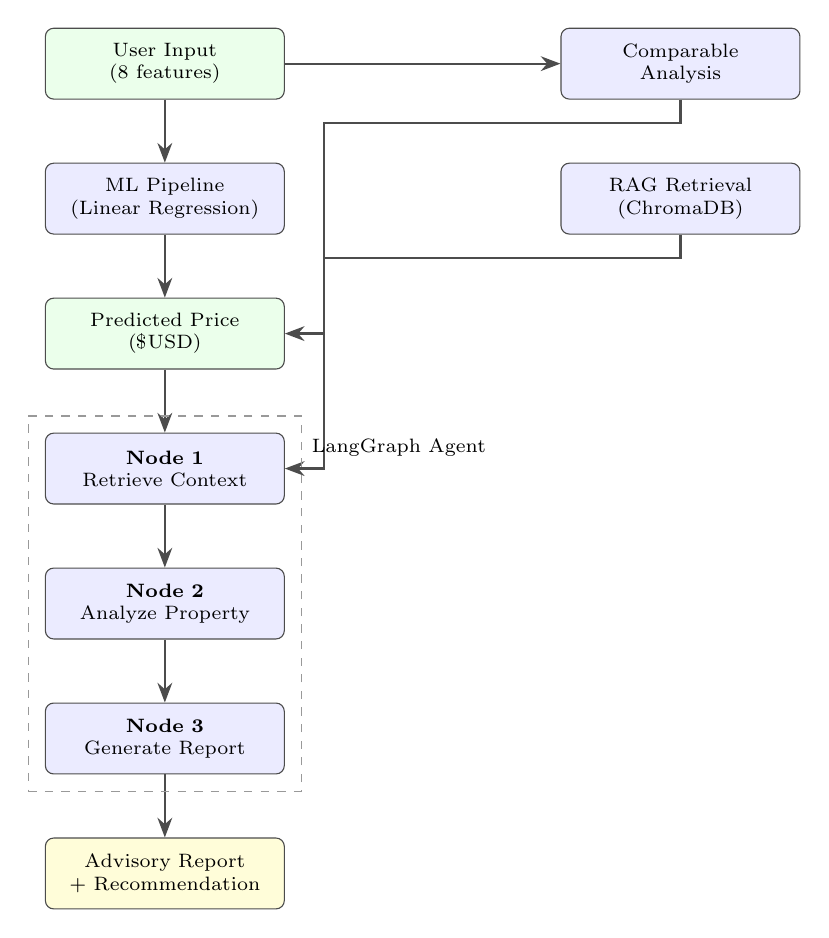
\begin{tikzpicture}[
    node distance=0.8cm and 1.0cm,
    block/.style={rectangle, draw=black!70, fill=blue!8, text width=2.8cm, minimum height=0.9cm, align=center, rounded corners=3pt, font=\scriptsize},
    data/.style={rectangle, draw=black!70, fill=green!8, text width=2.8cm, minimum height=0.9cm, align=center, rounded corners=3pt, font=\scriptsize},
    output/.style={rectangle, draw=black!70, fill=yellow!15, text width=2.8cm, minimum height=0.9cm, align=center, rounded corners=3pt, font=\scriptsize},
    arrow/.style={-{Stealth[length=2.5mm]}, thick, color=black!70},
]

\node[data] (input) {User Input\\(8 features)};
\node[block, below=of input] (ml) {ML Pipeline\\(Linear Regression)};
\node[data, below=of ml] (pred) {Predicted Price\\(\$USD)};

\node[block, right=3.5cm of input] (comps) {Comparable\\Analysis};
\node[block, right=3.5cm of ml] (rag) {RAG Retrieval\\(ChromaDB)};

\node[block, below=of pred] (n1) {\textbf{Node 1}\\Retrieve Context};
\node[block, below=of n1] (n2) {\textbf{Node 2}\\Analyze Property};
\node[block, below=of n2] (n3) {\textbf{Node 3}\\Generate Report};

\node[output, below=of n3] (report) {Advisory Report\\+ Recommendation};

\draw[arrow] (input) -- (ml);
\draw[arrow] (ml) -- (pred);
\draw[arrow] (input.east) -- ++(0.5,0) |- (comps.west);
\draw[arrow] (comps.south) -- ++(0,-0.3) -| ([xshift=0.5cm]pred.east) -- (pred.east);
\draw[arrow] (pred) -- (n1);
\draw[arrow] (rag.south) -- ++(0,-0.3) -| ([xshift=0.5cm]n1.east) -- (n1.east);
\draw[arrow] (n1) -- (n2);
\draw[arrow] (n2) -- (n3);
\draw[arrow] (n3) -- (report);

\node[draw=black!40, dashed, fit=(n1)(n2)(n3), inner sep=6pt, label={[font=\scriptsize]above right:LangGraph Agent}] {};

\end{tikzpicture}
}
\caption{End-to-end system pipeline from user input to advisory report.}
\label{fig:e2e}
\end{figure}

The pipeline executes in four sequential stages:

\begin{enumerate}[leftmargin=*]
    \item \textbf{ML Prediction (Step~1):} The user's feature inputs are transformed into a single-row DataFrame matching the training schema, then passed through the loaded scikit-learn pipeline to produce a price estimate in USD.
    \item \textbf{Comparable Analysis (Step~2):} The user's features are matched against the historical dataset to find similar properties and compute summary statistics.
    \item \textbf{Agent Execution (Step~3):} The LangGraph agent runs its three nodes sequentially---retrieving market context, analysing valuation, and generating the advisory report.
    \item \textbf{UI Rendering (Step~4):} The Streamlit frontend displays the predicted price, advisory report, evidence panel (retrieved context and comparables), and prediction history.
\end{enumerate}

% -------------------------------------------------
% 14. Streamlit Application
% -------------------------------------------------
\section{Streamlit Application}

\subsection{User Interface}

The Streamlit app provides a two-column layout:

\begin{itemize}[leftmargin=*]
    \item \textbf{Left column:} A prediction card showing the latest estimated price, input controls (sliders and number inputs) for eight key features, and Predict/Clear action buttons.
    \item \textbf{Right column:} A prediction history chart, the AI-generated advisory report (with sections for Valuation, Market Insights, Comparable Analysis, Recommendation, Risks, and Disclaimer), and a history table.
\end{itemize}

The application also provides \textbf{preset configurations} (Starter, Family, Premium) that pre-fill the input controls with representative property profiles, enabling quick exploration.

\subsection{Evidence and Transparency}

The UI includes an evidence panel that shows:

\begin{itemize}[leftmargin=*]
    \item \textbf{Retrieved market context:} The RAG-sourced domain insights used in the advisory.
    \item \textbf{Comparable properties:} The statistical summary of matched historical sales.
\end{itemize}

This transparency allows users to understand and verify the basis of the AI's recommendation.

% -------------------------------------------------
% 15. Integrated Results
% -------------------------------------------------
\section{Integrated Results and Discussion}

\subsection{ML Model Performance}

As reported in Section~\ref{sec:ml-eval}, the Linear Regression model with log-transformed target achieves strong predictive performance:

\begin{itemize}[leftmargin=*]
    \item \textbf{R\textsuperscript{2} = 0.9326}: The model explains 93.3\% of the variance in sale prices.
    \item \textbf{MAE = \$14,899}: On average, predictions deviate by approximately \$15K from actual prices, which is reasonable for the Ames housing market where median prices are approximately \$160K.
    \item \textbf{RMSE = \$22,740}: Larger errors (e.g., for luxury properties) contribute more to RMSE, but the overall magnitude remains acceptable.
\end{itemize}

\subsection{RAG Retrieval Quality}

The RAG system retrieves contextually relevant domain knowledge that grounds the advisory.
For a typical query about a high-quality, large-area property, the retriever returns insights about appreciation rates for quality homes, the relationship between living area and value, and investment considerations---all directly relevant to the advisory context.

\subsection{Agent Workflow Effectiveness}

The three-node agent workflow achieves its design goals:

\begin{itemize}[leftmargin=*]
    \item \textbf{Node 1 (Retrieval):} Successfully retrieves relevant market context from the vector store, providing the LLM with grounded evidence.
    \item \textbf{Node 2 (Analysis):} The $\pm$20\% valuation threshold provides a simple but effective heuristic for flagging over/undervalued properties relative to comparables.
    \item \textbf{Node 3 (Report Generation):} When the LLM is available, it produces well-structured, grounded advisory reports. When unavailable, the fallback generates consistent, rule-based reports that still provide actionable guidance.
\end{itemize}

\subsection{Advisory Report Quality}

The generated advisory reports follow a consistent structure:

\begin{enumerate}[leftmargin=*]
    \item \textbf{Property Valuation:} The ML-predicted price prominently displayed.
    \item \textbf{Market Insights:} Three RAG-sourced insights relevant to the property.
    \item \textbf{Comparable Analysis:} Summary of similar properties with valuation assessment.
    \item \textbf{Recommendation:} One of Buy / Wait / Caution with supporting reasoning.
    \item \textbf{Risks:} Two specific risk factors based on the valuation assessment.
    \item \textbf{Disclaimer:} Standard advisory disclaimer.
\end{enumerate}

Table~\ref{tab:advisory-examples} shows illustrative advisory outputs for different property profiles.

\begin{table}[H]
    \centering
    \caption{Illustrative advisory outputs for different property profiles.}
    \label{tab:advisory-examples}
    \begin{tabular}{llll}
        \toprule
        \textbf{Profile} & \textbf{Predicted Price} & \textbf{Valuation} & \textbf{Recommendation} \\
        \midrule
        Starter (Qual=4, 1100 sqft) & $\sim$\$100K & Fair/Undervalued & Buy \\
        Family (Qual=6, 1850 sqft)  & $\sim$\$175K & Fair & Wait \\
        Premium (Qual=8, 2850 sqft) & $\sim$\$310K & Fair/Overvalued & Caution \\
        \bottomrule
    \end{tabular}
\end{table}

% -------------------------------------------------
% 16. Limitations
% -------------------------------------------------
\section{Limitations and Future Work}

\subsection{Current Limitations}

\begin{itemize}[leftmargin=*]
    \item \textbf{Static knowledge base:} The RAG knowledge base consists of a small number of curated sentences. Real-time market data, news feeds, or regulatory updates are not incorporated.
    \item \textbf{LLM dependency:} The system relies on an external LLM API (OpenRouter). While the fallback mitigates this, the LLM-generated reports are richer and more nuanced.
    \item \textbf{Single dataset:} The model is trained on Ames, Iowa housing data and may not generalise to other markets without retraining.
    \item \textbf{Limited feature exposure:} Only 8 of the 79 features are exposed in the UI; the remaining features are zero-filled, which may affect prediction accuracy for properties that differ significantly in unexposed features.
    \item \textbf{No uncertainty quantification:} The ML model provides point estimates without confidence intervals.
\end{itemize}

\subsection{Future Work}

\begin{itemize}[leftmargin=*]
    \item \textbf{Richer RAG corpus:} Incorporate real-time property listings, market reports, and regulatory documents into the vector store.
    \item \textbf{Multi-agent validation:} Add a reviewer agent node that cross-checks the generated advisory against the evidence before returning the final report.
    \item \textbf{Advanced ML models:} Evaluate Gradient Boosting (XGBoost, LightGBM) and neural network approaches for potentially better predictive performance.
    \item \textbf{Explainability:} Integrate SHAP values or coefficient-based breakdowns to show which features most influenced each prediction.
    \item \textbf{Uncertainty bands:} Compute prediction intervals using validation residuals or conformal prediction methods.
    \item \textbf{Broader market coverage:} Extend to multiple housing markets with transfer learning or market-specific fine-tuning.
\end{itemize}

% -------------------------------------------------
% 17. Additional Design Choices
% -------------------------------------------------
\section{Additional Design Choices}

\subsection{Agent Design Choices}

\begin{itemize}[leftmargin=*]
    \item \textbf{Linear DAG over dynamic routing:} A fixed three-node sequence provides predictable latency and deterministic behaviour, which is preferred for a user-facing application.
    \item \textbf{Prompt engineering:} The LLM prompt uses strict formatting rules and explicit instructions to avoid hallucination, ensuring the advisory stays grounded in the provided evidence.
    \item \textbf{Response caching:} LRU caching of LLM responses avoids redundant API calls for identical property configurations.
    \item \textbf{Text cleaning:} A dedicated text cleaner normalises LLM output (fixing spacing, formatting headings, cleaning bullet points) for consistent UI rendering.
\end{itemize}

\subsection{Deployment Optimizations}

\begin{itemize}[leftmargin=*]
    \item \textbf{Single artifact:} The entire preprocessing + model pipeline is packaged into one joblib file.
    \item \textbf{Version pinning:} Critical library versions are pinned in \texttt{requirements.txt} (scikit-learn 1.6.1, joblib 1.5.3, numpy 2.0.2, pandas 2.3.3).
    \item \textbf{Progress feedback:} A Streamlit progress bar provides real-time feedback during the multi-step analysis (15\% $\rightarrow$ 35\% $\rightarrow$ 55\% $\rightarrow$ 80\% $\rightarrow$ 100\%).
\end{itemize}

% -------------------------------------------------
% 18. Technology Stack Summary
% -------------------------------------------------
\section{Technology Stack}

Table~\ref{tab:tech-stack} summarises the complete technology stack.

\begin{table}[H]
    \centering
    \caption{Technology stack and components.}
    \label{tab:tech-stack}
    \begin{tabular}{ll}
        \toprule
        \textbf{Component} & \textbf{Technology} \\
        \midrule
        Language & Python 3.10+ \\
        ML Framework & Scikit-learn 1.6.1 \\
        Data Processing & Pandas 2.3.3, NumPy 2.0.2 \\
        Model Serialization & Joblib 1.5.3 \\
        Vector Store & ChromaDB \\
        Embeddings & Sentence Transformers (all-MiniLM-L6-v2) \\
        LLM Gateway & OpenRouter API \\
        Agent Framework & LangGraph \\
        RAG Framework & LangChain (Community + HuggingFace) \\
        Web UI & Streamlit \\
        Version Control & Git / GitHub \\
        \bottomrule
    \end{tabular}
\end{table}

% -------------------------------------------------
% 19. Team Contribution
% -------------------------------------------------
\section{Team Contribution}

The project was a collaborative effort. Each team member had clearly defined responsibilities, which are summarised below.

\subsection*{Kavya Katal}

\begin{itemize}[leftmargin=*]
    \item Led \textbf{model training} and experimentation in the Jupyter notebooks.
    \item Designed and implemented the \textbf{preprocessing pipelines} using \texttt{ColumnTransformer} and \texttt{Pipeline}.
    \item Trained and evaluated the \textbf{Linear Regression} and \textbf{Random Forest} models.
    \item Contributed to the \textbf{technical report} and documentation of the modelling decisions.
\end{itemize}

\subsection*{Aabir Sarkar}

\begin{itemize}[leftmargin=*]
    \item Handled \textbf{data cleaning and preprocessing}, including handling missing values, column type checks, and dataset sanity validation.
    \item Implemented the \textbf{Streamlit application} logic, including loading saved artifacts, building input DataFrames, and running predictions.
    \item Designed and implemented the \textbf{LangGraph agent workflow}, \textbf{RAG pipeline}, and \textbf{LLM integration}.
    \item Wrote and refined the \textbf{LaTeX report}, integrating results from the notebook and codebase.
\end{itemize}

\subsection*{Kushagra Maheswari}

\begin{itemize}[leftmargin=*]
    \item Responsible for \textbf{dataset sourcing}, ensuring the correct Ames Housing dataset was obtained and integrated into the project.
    \item Created the \textbf{demo video} showcasing the model and the Streamlit app in action.
    \item Helped verify that the user interface behaved correctly for different input configurations.
\end{itemize}

\subsection*{Pratyush Chouksey}

\begin{itemize}[leftmargin=*]
    \item Contributed to \textbf{dataset sourcing} and validation of the raw data.
    \item Assisted in writing parts of the \textbf{project report}, especially sections related to data description and EDA.
    \item Helped cross-check the consistency between the notebook results and the deployed model.
\end{itemize}

% -------------------------------------------------
% 20. Conclusion
% -------------------------------------------------
\section{Conclusion}

This project demonstrates how Machine Learning, Retrieval-Augmented Generation, and agentic workflows can be integrated into a cohesive real estate advisory system.
The ML pipeline provides accurate price predictions (R\textsuperscript{2} = 0.93), the RAG system grounds the advisory in retrievable domain knowledge, and the LangGraph agent orchestrates the multi-step reasoning required to produce structured, actionable investment reports.

The system's three-node agent architecture---Retrieve, Analyse, Generate---reflects a principled separation of concerns, while the rule-based fallback ensures reliability regardless of external API availability.
Deployed as an interactive Streamlit application, the system makes the combined intelligence of statistical modelling and AI-augmented reasoning accessible to non-technical users.

Future directions include expanding the RAG knowledge base with real-time market data, adding multi-agent validation for report quality, integrating advanced ML models, and providing explainability through feature attribution methods.

\end{document}
